% Based on a template created by João Alegria (https://github.com/joao-alegria)
%  and Filipe Pires (https://github.com/FilipePires98)
 
\documentclass[12pt]{article}

\usepackage[english]{babel}
\usepackage[utf8x]{inputenc}

\usepackage{float}
\usepackage{hyperref}
\usepackage{times}
\usepackage{url}

% Images
\usepackage{graphicx}
\graphicspath{{images/}}

% Page dimensions
\topmargin -1.0cm
\oddsidemargin 0.0cm
\textwidth 16cm 
\textheight 23cm
\footskip 1.0cm

% TITLE PAGE CONTENT BEGIN

\title{Assignmnet 2}

\author{
    André Pedrosa [85098], João Abílio [84732]\\
    \\
    Recuperação de informação\\
    \normalsize{Departamento de Eletrónica, Telecomunicações e Informática}\\
    \normalsize{Universidade de Aveiro}\\
}

\date{13 de outubro de 2019}

% TITLE PAGE CONTENT END

\begin{document}

\baselineskip18pt

\maketitle

\section{Introdução}
Este relatório apresenta uma explicação do trabalho desenvolvido
para o segundo assignment da disciplina "Recuperação de Informação",
explicando as decisões tomadas e o funcionamento da solução.

Esta segunda entrega tem como objetivo fazer incrementos à entrega anterior
de maneira a aplicar o método SPIMI durante o método de indexação, aplicar
pesos td-idf aos termos usando o esquema de indexação {\it lnc.ltc} e adicionar
ao indexer as posições dos termos nos documentos nos quais ele aparece.

No fim serão apresentados a medidas de eficiência pedidas no enunciado do
assigment para cada novo método de indexação.

Devido ao elevado número de classes criadas, o diagrama de classes vai ser
dividido em vários que vão sendo apresentados ao longo do relatório. Estes
diagramas foram gerados através do IDEA IntelliJ, consequentemente em anexo
é disponibilizada a legenda da convenção usada.

\section{Data Flow}
\begin{figure}[h]
  \center
  \includegraphics[width=\linewidth]{newsequenceDiagram.png}
  \caption{Diagrama de sequência da solução}
  \label{fig:dataflow}
\end{figure}

O data flow da nossa solução, de modo geral não sofreu grandes
alterações, apenas migramos o código de execução da pipeline de
indexação para uma classe separada, em vez de ser definida na
classe Main.

Na figura \ref{fig:dataflow} está representado sequência de execução
da nossa solução, onde as setas azuis significam que a classe origem
executa um método da classe destino e as setas vermelhas significam
que a classe origem cria a classe destino. Deixando de parte as classes
que têm uma seta vermelha a apontar para si, todas as classes são
instanciadas na classe Main. Na figura existem várias classes em que é
apresentado a classe base e a sua implementação, isto pois algumas
classes base apresentam métodos {\it final} que chamam depois métodos
abstratos que devem estar definidos em classes de descendentes (padrão
Template Method).

\section{Packages}
\begin{figure}[H]
  \center
  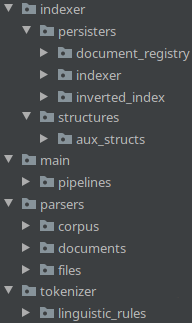
\includegraphics[width=6cm]{packages_all.png}
  \caption{Árvore de packages da solução}
\end{figure}

Nesta secção vão ser apresentadas as alterações feitas a cada package
relativamente à entrega anterior.

\subsection{main}

\begin{figure}[h]
  \center
  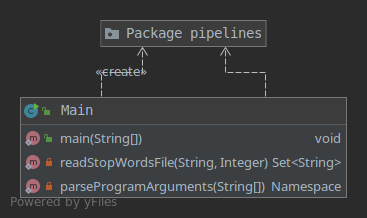
\includegraphics[width=6cm]{packages_main.png}
  \caption{Diagrama de classes do package \it main.pipelines}
\end{figure}


Como foi dito na secção anterior, o código de execução da pipeline
de indexação que estava presente na classe Main, foi migrado para
para uma classe do tipo Pipeline. Ou seja, a classe Main apenas
tem a responsabilidade de instanciar as classes necessárias para
a execução da pipeline.

\subsubsection{pipelines}

\begin{figure}[h]
  \center
  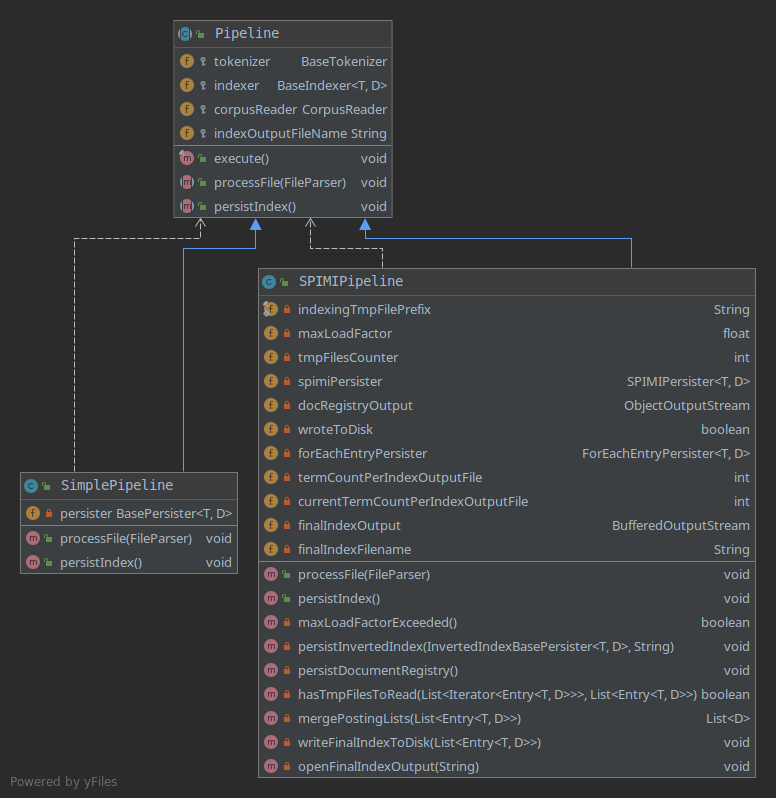
\includegraphics[width=\linewidth]{packages_main_pipelines.png}
  \caption{Diagrama de classes do package \it main.pipelines}
\end{figure}

Este package tem as classes que definem a sequência de execução
do método de indexação. A classe principal (Pipeline) está encarregue
de iterar sobre o corpus e passar cada FileParser à implementação
de Pipeline escolhida (método processFile) e depois disso executar
o método para persistir o indexer.

A classe SimplePipeline representa a pipeline que foi definida no
assignment anterior, em que não tem considerações relativamente à
memória no processo de indexação. A SPIMIPipeline apresenta uma
implementação em que o método de indexação é feito segundo o
algoritmo SPIMI, em que durante a indexação, sempre que a memória
ocupada chegar a um limite, o index atual é escrito para disco, ordenado
pelos termos. Na altura de persistir o index, esta pipeline faz um merge
dos vários ficheiros criados na fase anterior. Este merge é feito lendo
blocos (implementado com a classe BufferedInputStream) de todos os
ficheiros temporários criados. Para fazer merge destes blocos, é mantida
uma lista à qual é adicionada iterativamente a entry (termo e posting
list) em que o termo é menor (alfabeticamente). Caso haja o mesmo termo
em diferentes blocos é feito o merge das posting lists segundo
os document ids.

Os ficheiros temporários foram escritos em binário (usando a class
ObjectOutputStream), já que se revelou ser muito mais rápido do que
aplicar a forma de persistência que o utilizador escolhe no Main, no
caso deste assignment CSV. Para guardar o index final foram criados
vários ficheiros, tendo cada um um número máximo de entries e para
saber quais os termos presentes em cada ficheiros deste foi inserido
como sufixo ao nome dos ficheiros o primeiro termo que guardam.

% TODO falar sobre o document registry

\subsection{parsers}
\begin{figure}[H]
  \center
  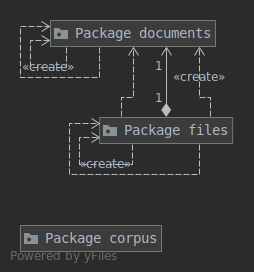
\includegraphics[width=\linewidth]{packages_parsers}
  \caption{Diagrama de classes do package \it parsers}
\end{figure}

Este package não sofreu grandes alterações relativamente à entrega
anterior, apenas foi alterado algumas mensagens de erro, os id dos
documentos agora começa em 0 e algumas operações sobre strings,
que não alteram o resultado final, obtidas dos ficheiros do corpus
foram removidas, como .trim(), para tentar reduzir o número de
instanciações da classe String.

\subsection{tokenizer}
\begin{figure}[H]
  \center
  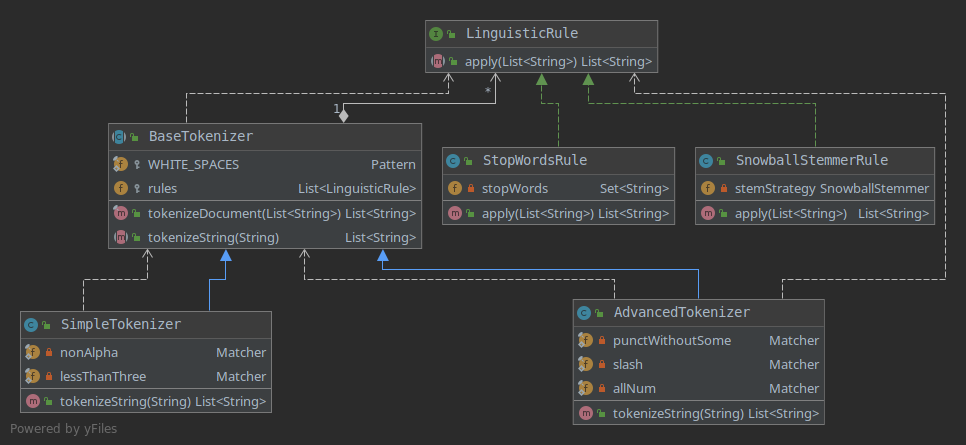
\includegraphics[width=\linewidth]{packages_tokenizer.png}
  \caption{Diagrama de classes do package \it tokenizer}
\end{figure}

Este package também não sofreu grandes alterações relativamente à
entrega anterior, apenas foi criada uma nova Linguistica Rule que
remove os termos que têm menos de um certo número de caracteres.

\subsection{indexer}
\begin{figure}[h]
  \center
  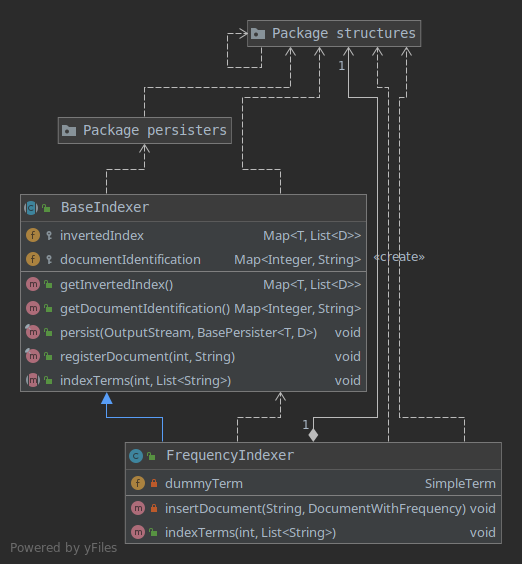
\includegraphics[width=8cm]{packages_indexer.png}
  \caption{Diagrama de classes do package \it indexer}
\end{figure}

Package com as classes que armazenam em memória o index invertido e
a associação entre o id de um documento e o seu identifier.

Aqui está presente a class BaseIndexer que serve como classe base para
diferentes implementações de indexers. O index invertido é guardado numa
estrutura do tipo mapa, permitindo ao programador definir a implementação
desta interface, sendo por defeito usado um HashMap. A classe base referida
é genérica o que possibilita que sejam criados diferentes indexers com a
mesma estrutura, o que leva às classes descendentes a implementar o método
{\it indexTerms} que guarda os termos de um documento no index invertido,
com as estruturas especificas desse indexer.

\subsubsection{indexer.structures}
\begin{figure}[h]
  \center
  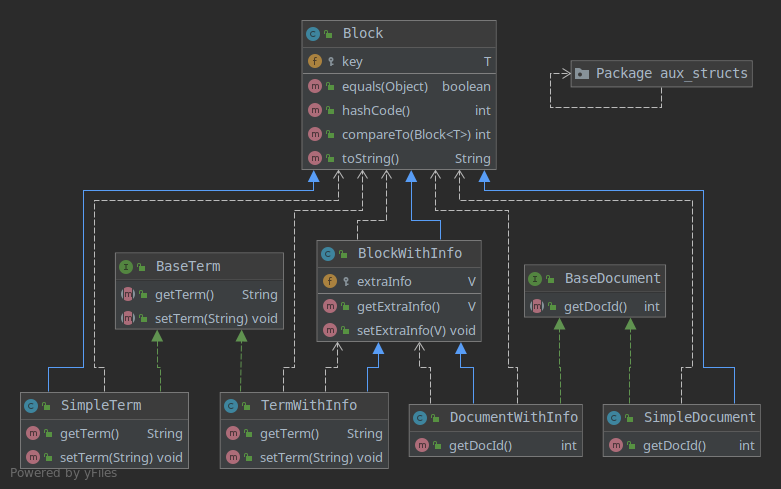
\includegraphics[width=10cm]{packages_indexer_structures.png}
  \caption{Diagrama de classes do package \it indexer.structures}
\end{figure}

Neste package estão os blocos que constroem o index invertido e que permitem
a extensibilidade do mesmo. Tanto a chave do index invertido como o valor presente
na lista associada descende do tipo Block que possui uma key (no caso do termo é o
próprio term e nos documentos o seu id) pela qual é comparável entre si. Em casos
em que seja necessário ter mais informação associada (contagens por exemplo)
a classe BlockWithInfo, descendente de Block, permite isso mesmo.

Para distinguir termos de documentos foram criadas as interfaces BaseTerm e BaseDocument,
logo classes que guardam informação sobre termos devem descender do tipo Block e
implementar a interface BaseTerm e classes que guardam informação sobre documentos
devem descender do tipo Block e implementar a interface BaseDocument.

\subsubsection{indexer.persisters}
\begin{figure}[H]
  \center
  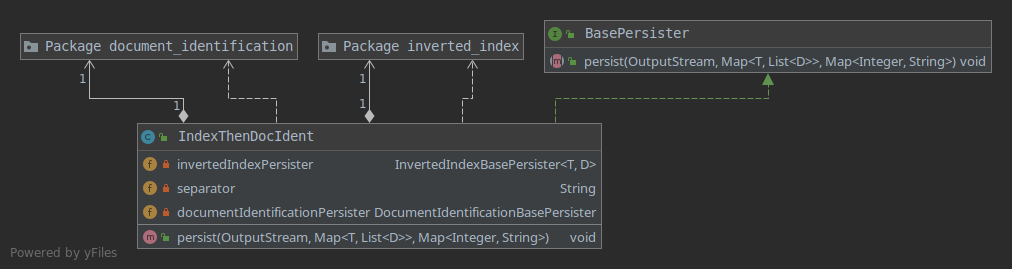
\includegraphics[width=16cm]{packages_indexer_persisters.png}
  \caption{Diagrama de classes do package \it indexer.persisters}
\end{figure}

Aqui encontram-se as classes responsáveis por implementar as diversas
estratégias de guardar as estruturas internas da class BaseIndexer
para disco. Como este indexer apresenta duas estruturas internas,
damos a possibilidade de criar diferentes estratégias para cada
estrutura, assumindo sempre que guardamos para o mesmo ficheiro as
duas estruturas. A classe BaseIndexer, no método {\it persist},
recebe um BasePersister que irá aplicar a estratégia para guardar
ambas as estruturas.

\begin{figure}[h]
  \center
  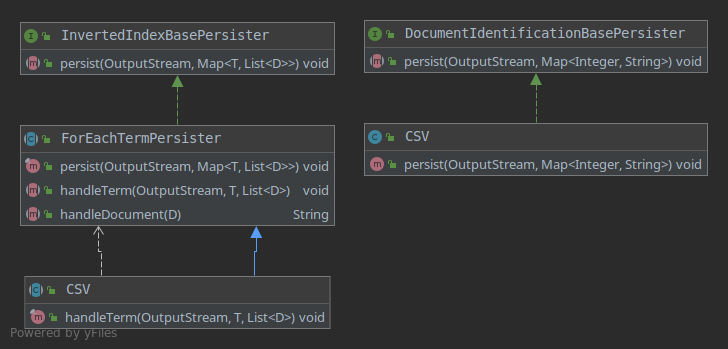
\includegraphics[width=16cm]{packages_indexer_persisters_impl.png}
  \caption{Diagrama de classes do package {\it indexer.persisters.inverted\_index}
  à esquerda e do package \it indexer.persisters.document\_identification
  à direita}
\end{figure}

\newpage

\section{Resultados}

Resultados usando apenas o ficheiro 2004\_TREC\_ASCII\_MEDLINE\_1.gz \\

\begin{tabular}{| p{0.4\linewidth} | p{0.3\linewidth} | p{0.3\linewidth} |}
        \hline
        & \bf SimpleTokenizer & \bf AdvancedTokenizer \\ \hline
        Tempo de indexação (mm:ss) & 3:13 & 2:09 \\ \hline
        Tamanho do index em disco (MB) & 238 & 209 \\ \hline
        Tamanho do vocabulário & 254914 & 427035\\ \hline
        Primeiros 10 termos (em ordem
        alfabética) que aparecem em
        apenas um documento
        &
        aaaa \newline
        aaaai \newline
        aaaasf \newline
        aaaat \newline
        aaab \newline
        aaact \newline
        aaaction \newline
        aaaga \newline
        aaah \newline
        aaahc
        &
        000case \newline
        000diseasegen \newline
        000for \newline
        000g \newline
        000gener \newline
        000iu \newline
        000kb \newline
        000mer \newline
        000meter \newline
        000molecularweight
        \\ \hline
        Dez termos com a maior frequência nos documentos
        &
       and : 1014861 \newline
       the : 1011732 \newline
      with : 311814 \newline
       for : 304357 \newline
      from : 117323 \newline
  patients : 112027 \newline
     human : 106054 \newline
      cell : 90208 \newline
     cells : 85435 \newline
     study : 84058
     &
      cell : 144666 \newline
   patient : 137526 \newline
    effect : 134752 \newline
     human : 109488 \newline
     studi : 106189 \newline
       use : 87725 \newline
     activ : 87489 \newline
       rat : 81501 \newline
    diseas : 79692 \newline
 treatment : 78885
     \\
    \hline
\end{tabular}
\newpage

\section{Anexos}

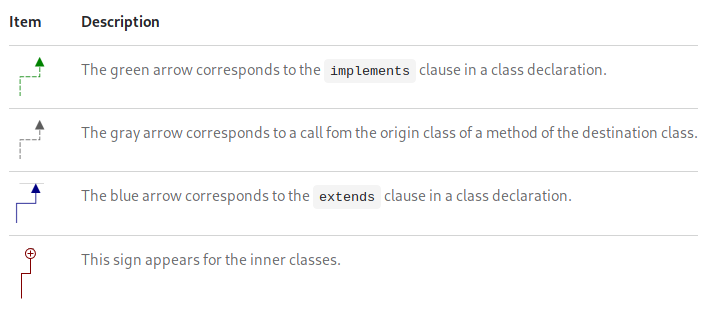
\includegraphics[width=13cm]{arrow_legend.png}

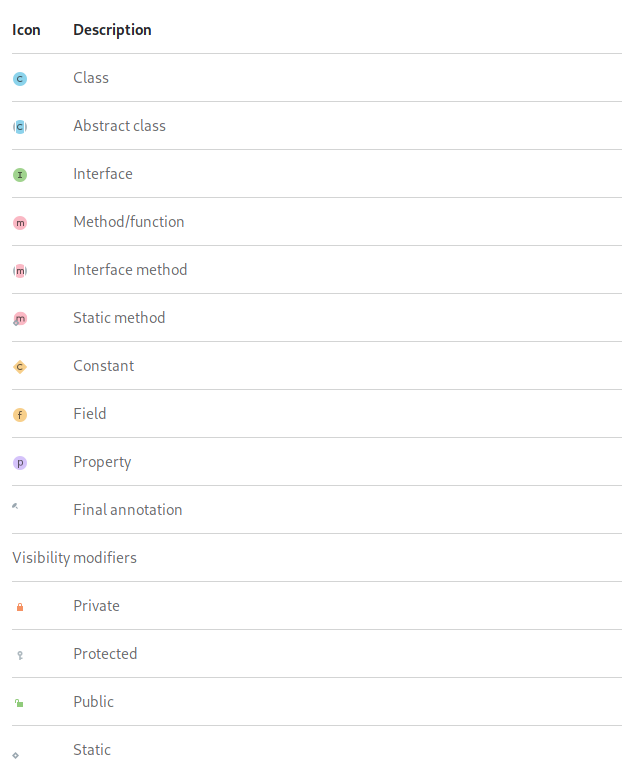
\includegraphics[width=13cm]{icons_legend.png}

\end{document}
